\testCom
{%Номер задачи
	3.138
}
{%Условие
	условие
}
{%Дано
	дано
}
{%Найти
	найти
}
{%Решение
	%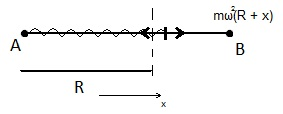
\includegraphics[height=30mm]{3_33.jpg}\\
	Очевидно, что контур теряет энергию из-за активного сопротивления (тепло) и эти потери описываются уравнением вида:\\
	$\der{Q}{t}{} = I^2 R$ - (закон Джоуля-Ленца), тогда искомая мощность $P = \der{Q}{t}{}, a \avr{P} = \frac{1}{T} \int\limits_0^T Q' \, dt$\\
	$I(t) = I_m \sin \omega t$ (гармонические колебания тока), тогда $T = \frac{2 \pi}{\omega}$\\
	$\avr{P} = \avr{I^2 (t) R} = R \frac{\omega I_m^2 }{2 \pi} \int\limits_0^{\frac{2 \pi}{\omega}} \sin^2 \omega t \, dt = R \frac{\omega I_m^2 }{2 \pi} \int\limits_0^{\frac{2 \pi}{\omega}} \frac{1 - \cancelto{0}{\cos \omega t}}{2} \, dt = \frac{I_m^2 R}{2}$\\
}

